\chapter{\IfLanguageName{dutch}{Stand van zaken}{State of the art}}
\label{ch:stand-van-zaken}

% Tip: Begin elk hoofdstuk met een paragraaf inleiding die beschrijft hoe
% dit hoofdstuk past binnen het geheel van de bachelorproef. Geef in het
% bijzonder aan wat de link is met het vorige en volgende hoofdstuk.

% Pas na deze inleidende paragraaf komt de eerste sectiehoofding.

As mentioned in the previous chapter, this research will go deeper into headless Drupal and attempt to figure out how to utilise it and why it became so popular. But before anwsering these questions it is important to have a clear understanding of what headless Drupal acually is. This will be discussed in this chapter. 

\section{Architectures}
A traditional CMS like Drupal in its base form consists of a monolithic architecture. This means that the CMS offers anything a user would need in a web application, including a database, back-end and front-end.

When going headless, the architecture of the CMS goes from monolithic to the so-called decoupled architecture. In this form, only the back-end and database that the CMS offers are utilised. Then, instead of distributing the content in this back-end to one channel, it can be consumed by different channels, including web applications made with front-end frameworks like React and Angular, but even mobile applications.

Monolithic and decoupled are the two main architectures that are considered when using a CMS, but there are two other architectures worth mentioning: the fully decoupled static site and progressively decoupled ~\autocite{Dropsolid2021}. All of these architectures will be discussed in this chapter.

\subsection{Monolithic or Traditional}
The traditional or monolithic architecture is the one used by all traditional CMSs out of the box. It means that the application is one big end-to-end system. For Drupal in particular, this means that the theming functions which encompass the front-end are completely coupled and dependent on Drupal's back-end.

This architecture has both upsides and downsides. One big upside is that this is a very robust and reliable system. The system is predictable and easy to use. The downside to this architecture is that it has led to something often called Drupalisms on the front-end ~\autocite{So2018}. This means that some terminology and features specific to Drupal came to exist, which are hard to understand for developers less familiar with Drupal. 

One other negative is that this system can feel limiting for front-end developers, because they have to work within the boundaries of the specific theme they are using.

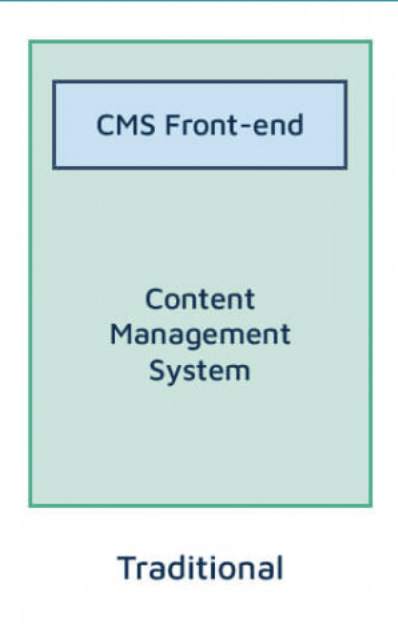
\includegraphics{./img/Traditional_Architecture}

\subsection{Headless or Decoupled}

The fully decoupled or headless architecture is the one that has become more and more popular over the years ~\autocite{Dropsolid2021}.

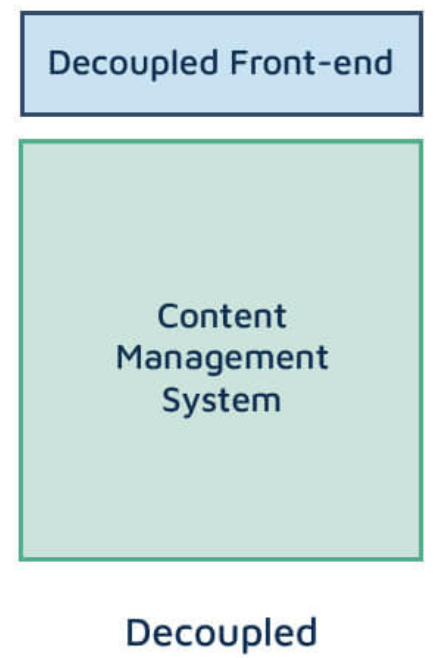
\includegraphics{./img/Headless_Architecture}

\subsection{Fully decoupled static site}

\subsection{Progressively decoupled}